\documentclass{report}
\usepackage[utf8]{inputenc}
\usepackage[french]{babel}
\usepackage{placeins}
\usepackage{graphicx}

\usepackage{amssymb}
\usepackage{amsmath}

\title{Rapport: Circuits RLC en tension carrée et sinusoïdale}
\author{Mattens Simon, Dom Eduardo \\ BAB2 Sciences Informatiques}
\date{26 avril 2018}
\begin{document}
\maketitle

\section*{1. Introduction}

\hspace*{0,5cm} Le  but  de  la  manipulation  est  l'étude  de  circuits  alimentés  en  tension  alternative 
(carrée  et 
sinusoïdale) 
comprenant 
des  associations  de  résistances  (R),  condensateurs  (capacités  C)  et 
bobines d'induction (L).

\section*{2. R\'esum\'e th\'eorie}
\subsection*{2.1 Rappels th\'eoriques n\'ecessaires aux calculs}
$\bullet$ Résistance  R "pure"  ou  résistance    ohmique  : élément  qui  "s'oppose"  au  passage  du courant  I tel que il y a proportionnalité entre la tension appliquée à ses bornes et le courant qui le traverse:     
$$ U_{R} = R.I$$
$\bullet$ Condensateur de capacité C : élément qui permet de stocker une quantité de charges proportionnelle à la tension appliquée à ses bornes : $ Q = CU  $
$\bullet$ Bobine  d'induction:  la  variation  d'un  courant  I  dans  une bobine  de  n  spires  conduit  à  un changement  du  flux  magnétique  la traversant donc induit  une  tension  aux bornes de cette bobine proportionnelle à la variation de courant : $$U_{L} = -L\frac{dI}{dt} $$
\\ Où l'inductance  L est  une  propriété  de  la  bobine,  facteur  de proportionnalité  entre  la  tension induite  et  la  variation  de  courant.

\section*{3. Manipulation}
\subsection*{3.1 Etude théorique d'un circuit (R)LC : oscillations sinusoïdales}
Considérons un circuit  LC  avec  L  =  0,1H  et  C  =  4300 pF.
Calculons la valeur de la période d’oscillation propre du circuit. \\

$$ T =  \frac{2 \pi}{\omega_{0}} = 2 \pi \sqrt{LC} = 1,30 . 10^{-4}s$$ \\

En tenant compte  de la  résistance  du  générateur (RG =  50 $\Omega$) et  de  celle de  la  bobine  (à mesurer): $ R_{L} = 65.3 \ \pm \ 0.66 \Omega \ $ (erreur de mesure).
On sait que $R=\frac{R_L.R_G}{R_L+R_G} $ pour un circuit LC en parallèle donc :
$R=\frac{65,3.50}{65,3+50} = 28.32\Omega$.
D'après cela, on peut calculer le temps de relaxation $\tau = \frac{2L}{R}=\frac{2.0,1}{28.32}=7,062.10^{-3}$s.

\subsection*{3.2 Circuit RLC série en tension carrée: mesures en régime transitoire}
1) La période du signal carré (répétition du phénomène ON - OFF): $T_{GS}$ = 9.94ms. \\
2) La période des oscillations : $T_{0}$ = 66.5ms.\\
3) Le temps de demi-vie de l'enveloppe exponentielle des amplitudes : $T_{1/2} = 157 \mu s$. \\
4) Donc , le temps de relaxation $\tau = 226.5 \mu s$ . \\
5) En examinant le schéma  du circuit, on détermine la valeur de $R_{TOT} = 560 + 65.9 + 50 = 675.9 \Omega$. On ne doit pas tenir compte de la résistance de l'oscillo car aucun courant ne passe par l'oscillo. \\
6) Ci-dessous, le tableau contenant les différents nombres d'oscillations observées en remplaçant la résistance de 560$\Omega$ par des résistances de valeurs différentes. \\

\begin{tabular}{|c|c|c|c|c|}
  \hline
  R = & 22$\Omega$ & 216$\Omega$ & 560$\Omega$  & 1500$\Omega$ \\
  \hline
  Nombre d'oscillations observées & 40.5 & 27.3 & 16.3 & 8.09 \\
  \hline
\end{tabular}
\subsubsection*{3.3 Étude du circuit RLC série en tension alternative sinusoïdale : résonance}
Nous avons pris des mesures  de la tension aux bornes du condensateur et son déphasage par rapport à la tension fournie par le générateur en faisant varier la fréquence de 100Hz à 3000Hz par pallier de 50 Hz,100 Hz,200 Hz,300 Hz(R vallant $22\Omega$ et $220\Omega$).
\hspace*{0.5cm}
\begin{figure}[ht!]
\centering
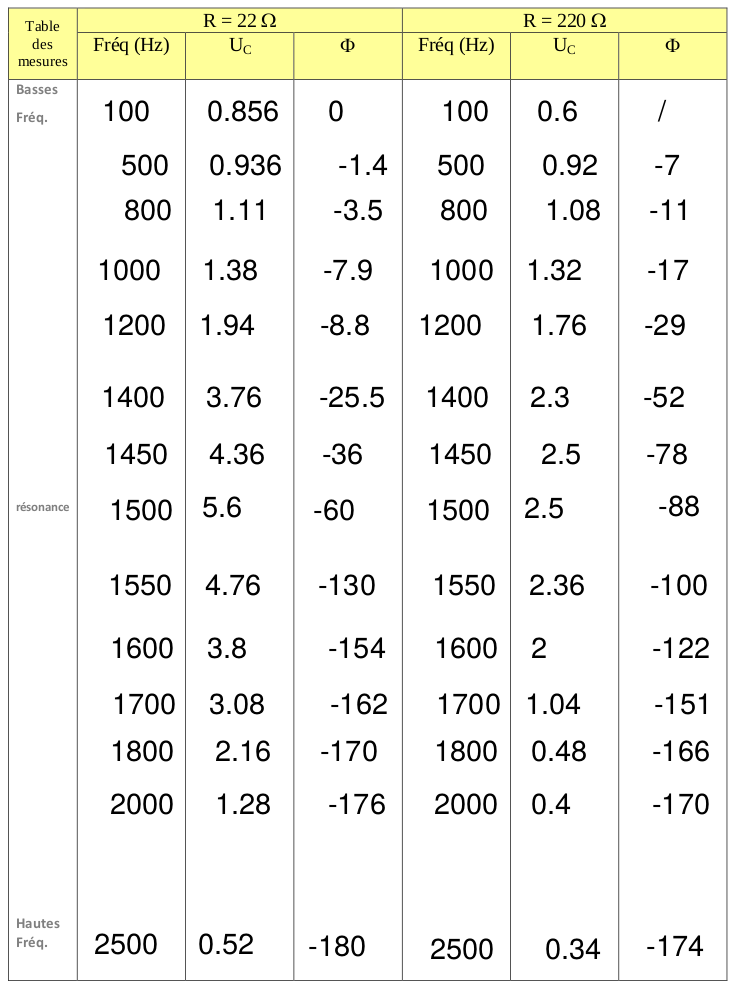
\includegraphics[width=150mm]{tableau.png}
\label{overflow}
\end{figure}
\FloatBarrier

\section*{4. Analyse des résultats}
\subsection*{4.1 Circuit RLC série en tension carrée}
Il nous est demandé d'examiner le schéma du circuit et de déterminer la valeur de $R_{tot}$ .
Via le multimètre, on a  obtenu la résistance de la bobine : $R_L=65,9\ \pm0,66\ \Omega$(erreur de mesure).$R_{tot}=R_R+R_L+R_G$ pour un circuit RLC en série donc : \\
\hspace*{5cm} $R_{tot}=560+65,9+50=675,9\Omega$\\
On ne doit pas tenir compte de la résistance de l'oscilloscope en parallèle car sa résistance est quasiment nulle , aucun courant ne passe par l'oscilloscope.\\
À présent nous devons calculer la valeur de l'inductance de la bobine L à partir des 2 résultats de mesure de $T_0$ et $\tau$ et comparer les 2 valeurs de L obtenues.\\ À partir de l'énoncé ,des mesure de $T_0$ et $\tau$, et sur base de C et $R_{tot}$ on peut calculer l'inductance de la bobine de deux manières:\\
\hspace*{2cm}(1)$L=\frac{\left({\frac{T_0}{2\pi}}\right)^2}{C} \Leftrightarrow $$ \ L = \frac{{\left(\frac{66,5.10^{-6}}{2\pi}\right)}^2}{10^{-9}}=0,112\ \Omega$
\\
\hspace*{2cm}(2)$L=\frac{\tau .R_{tot}}{2} \ $$ \Leftrightarrow $$ \ L=\frac{226,5.10^{-6}.675,9}{2}=0,076\ \Omega$\\
Ensuite , il nous est demandé de déterminer les fréquences de résonance pour les 2 résistances en se demandant si,théoriquement,ces fréquences devraient différer.
Pour cela nous avons fait varier la fréquence du générateur et mesuré  la tension aux bornes du condensateur et le déphasage. Nous
avons trouvé la même fréquence de résonance,valant 1500 Hz, pour les deux résistances.  Donc ces fréquences ne devraient pas différer.

\section*{5. Conclusion}
Nous avons étudié le comportement de deux circuits RLC disposés
différemment : l'un en série pour lequel nous avons étudié la tension aux bornes du condensateur.Et l’autre en parallèle pour lequel nous avons étudié le phénomène de résonance.

\end{document}
